\documentclass[tikz]{standalone}
\usetikzlibrary{decorations.pathmorphing}

% https://tex.stackexchange.com/questions/198057/tikz-drawing-railway-tracks

\tikzstyle{track}=[
    postaction={draw=gray,densely dashed,line width=14pt},
    postaction={draw,decorate,decoration={curveto,raise=4pt},line width=2pt},
    postaction={draw,decorate,decoration={curveto,raise=-4pt},line width=2pt}]

\begin{document}

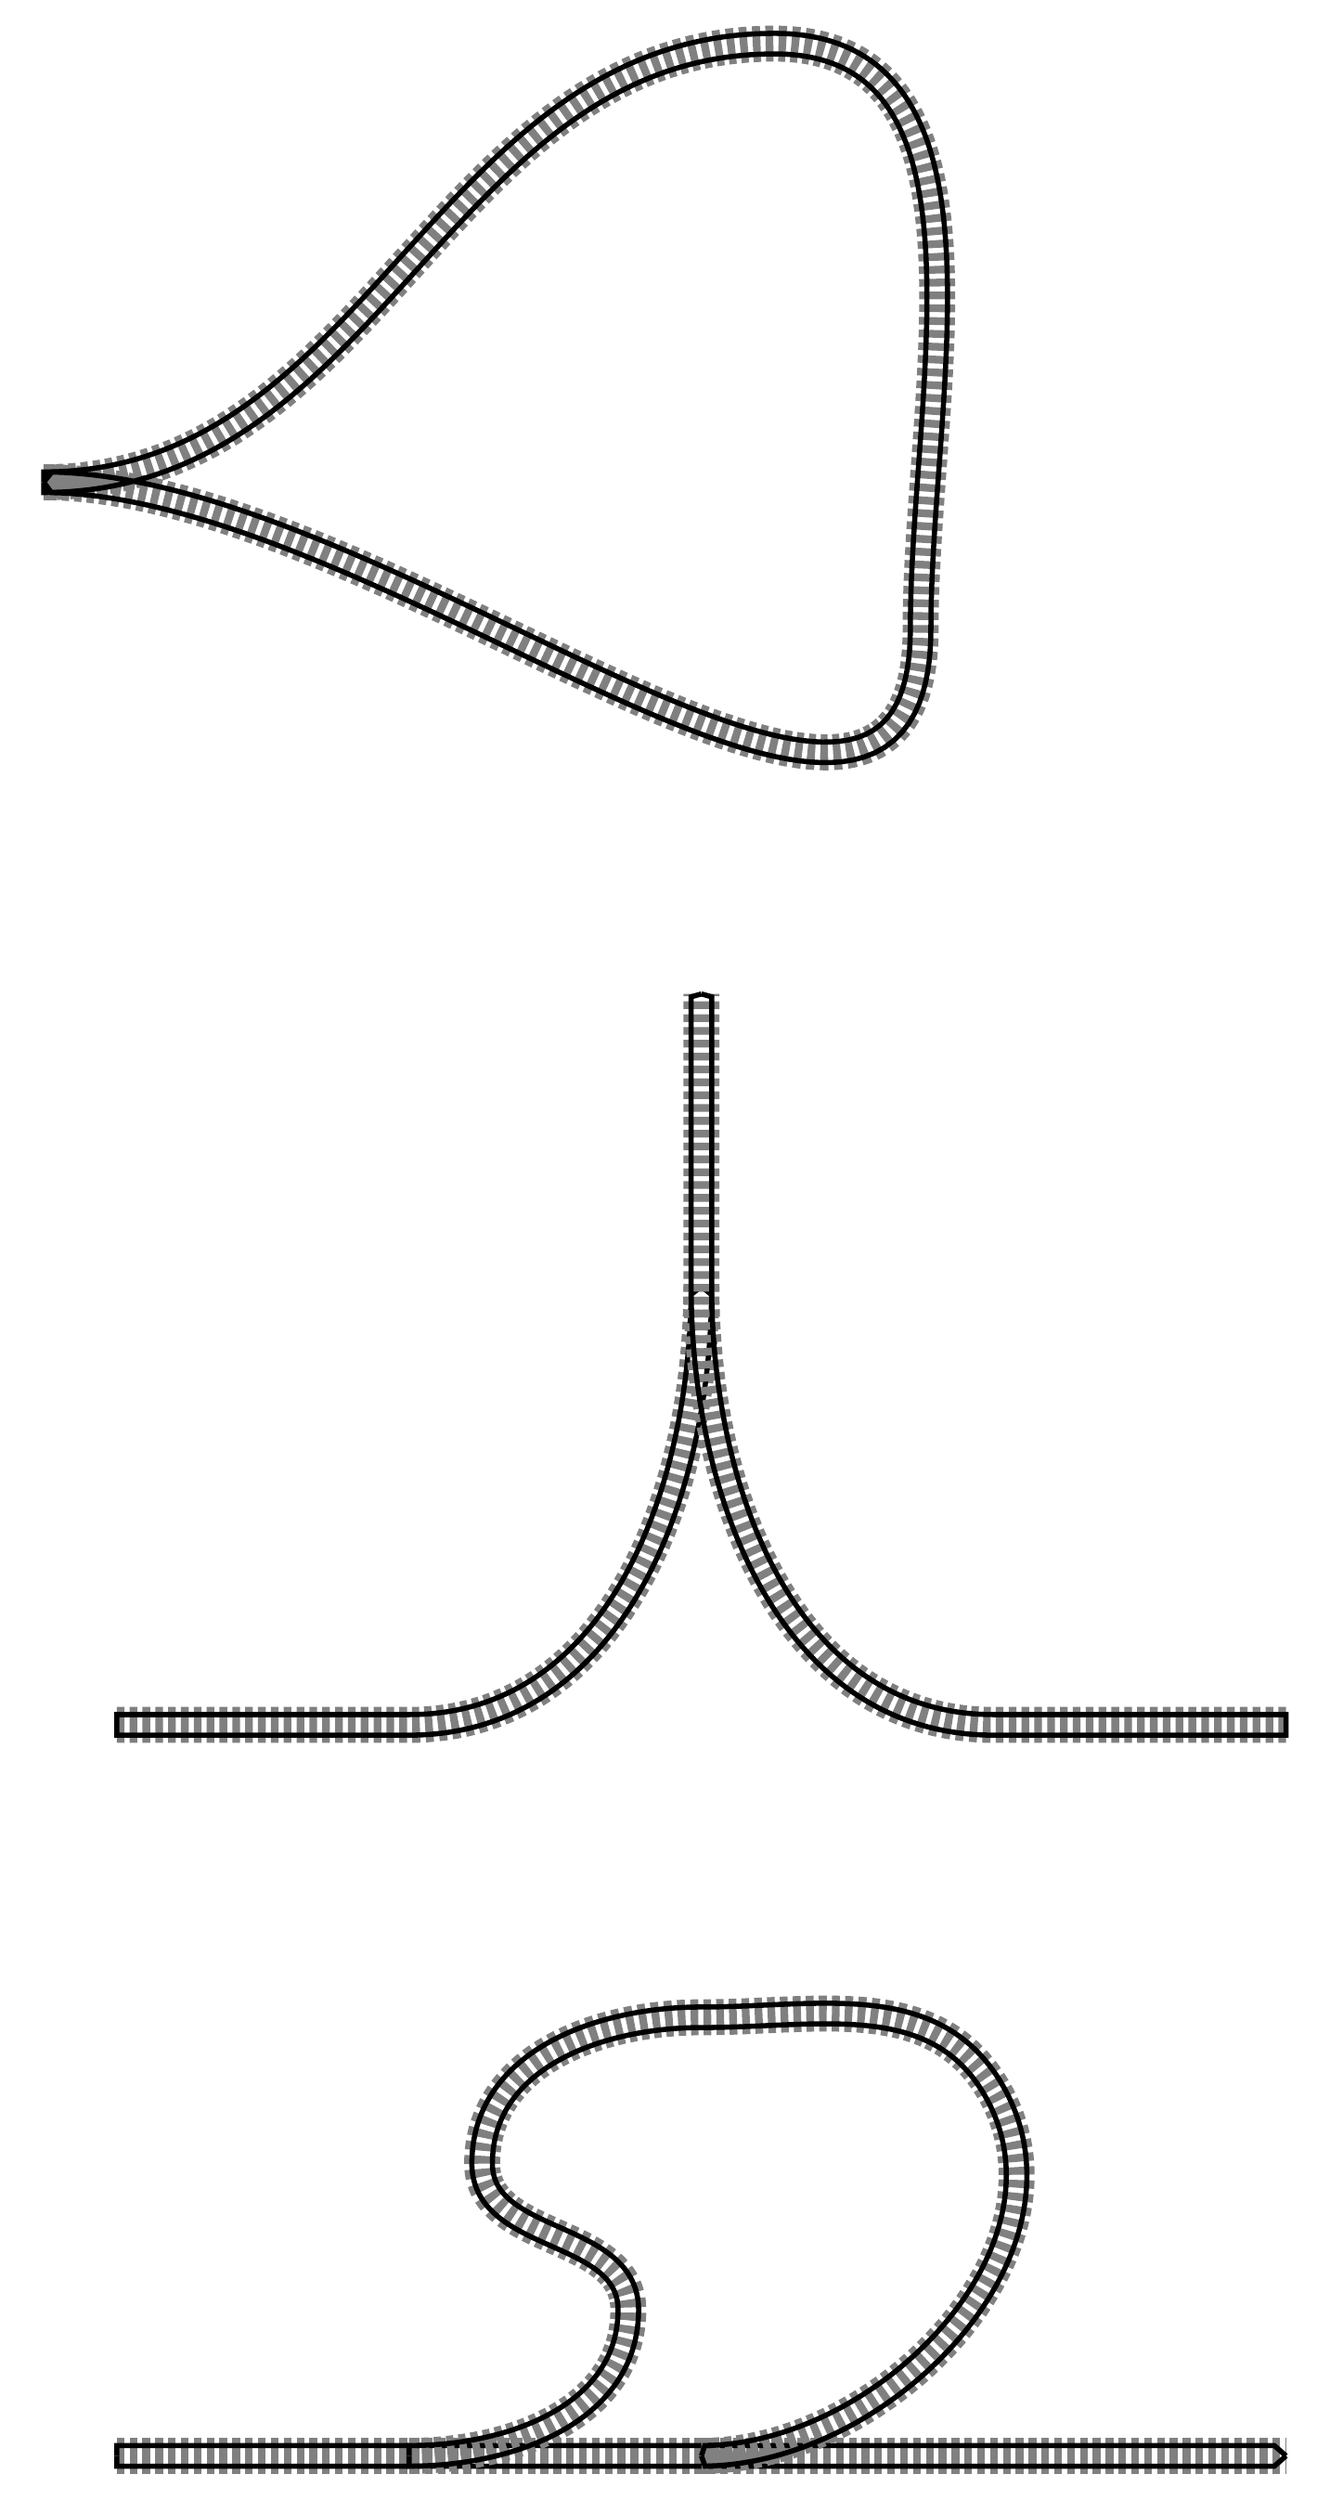
\begin{tikzpicture}

    \path[track] (-5,27)    to[out=  0,in=180] ( 5,33) 
                            to[out=  0,in= 90] ( 7,25) 
                            to[out=270,in=  0] (-5,27);

    \path[track] (-4,10)    to ( 0,10) to[out=  0,in=270] (4,16);
    \path[track] (12,10)    to ( 8,10) to[out=180,in=270] (4,16) to (4,20);

    \path[track] (-4, 0)    to (12, 0);

    \path[track] ( 0, 0)    to[out=  0,in=270] (3,2) 
                            to[out= 90,in=270] (1,4)
                            to[out= 90,in=180] (4,6) 
                            to[out=  0,in=120] (8,5) 
                            to[out=300,in=  0] (4,0);
\end{tikzpicture}

\end{document}
